\myChapter{Introduction}\label{chap:introduction}
\begin{flushright}{\slshape
    .} \\ \medskip
    --- {}
\end{flushright}
\minitoc\mtcskip
\vfill



\section{Goals of this Thesis} 

\lettrine{T}{he} goal of this thesis is to develop a methodology of data preprocessing, behaviour analysis, and consequent rule creation in a Bring Your Own Device (BYOD) context. This methodology proposes using a combination of Data Mining (DM) and Soft Computing (SC) techniques %Pablo: Habría que dejar clara la diferencia entre los dos en algún sitio en la intro, o quizás solo centrarse en un término.
% He cambiado ML por data mining a ver si así queda mejor. Pablo: Uuuuhm, sigo dándole vueltas a ver cuando Maribel te lo revise qué opina. Es que es un follón las definiciones de cada cosa, porque es casi todo lo mismo xD
 over context information related to a user interacting with a device, making benefit of the feature of rule model creation in some of these techniques. As a validation of this methodology, we will use it to help evolving an initial, simple, and fixed set of security rules into a new set of rules that will aid in the discovery of dangerous situations.

\section{Motivation}
\label{sec:intro:byod}

\lettrine{T}{he} fast pace of introduction of new technologies, including the so-called \textit{smart devices}, has led modern computing to move in a short period of time to smaller, more reliable, and faster devices such as smartphones, laptops, and tablets. At the same time, the use people give them is more varied and, among others, has given birth to the form of use known as the ``Bring Your Own Device'' (BYOD) concept or philosophy. Its first appearance as a concept was in research \cite{ballagas2004byod} as a way to name the interaction between people's devices and a public display, for instance, an advertising where people translate a QR code with their devices that takes them to a commercial website. Since then, it has become a very popular practise, integrated into companies \cite{thomson2012byod} and even schools \cite{song2014bring}. Also, researchers have continued to study the possibilities of this philosophy, as well as its problems and ways of integrate it in the different environments. Figure \ref{fig:pperyear} shows the number of indexed papers in the Scopus \footnote{\url{http://www.scopus.com}} database per year, when the terms {\em ``bring your own device'' OR byod} are included in the search.

\begin{SCfigure}[tb]
	\centering
	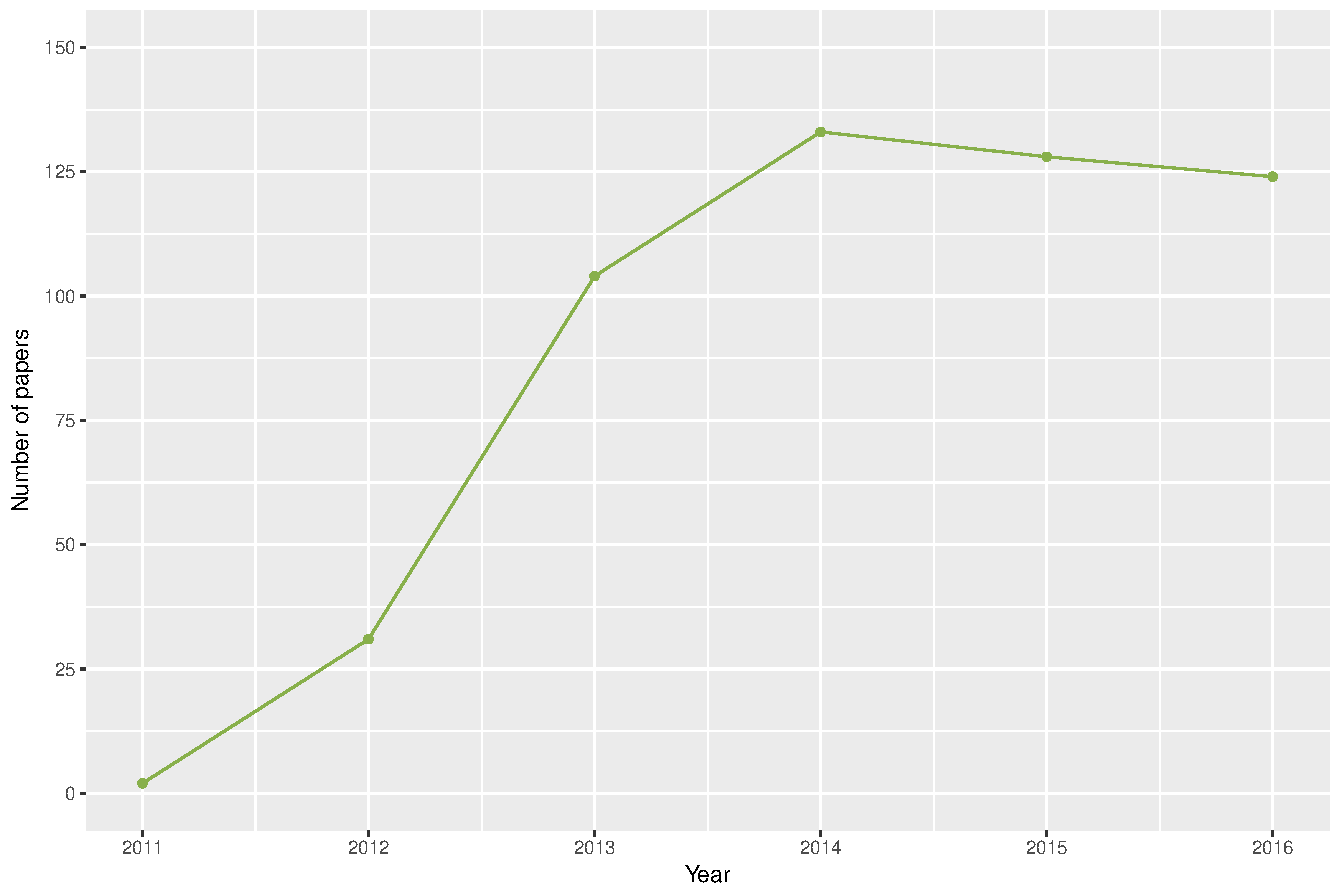
\includegraphics[scale =0.5] {gfx/intro/BYODpapers_year.pdf}
	\caption{Published papers per year in the BYOD topic. Data gathered from the Scopus database.}
	\label{fig:pperyear}
\end{SCfigure}

More precisely, in the corporate world the BYOD practice refers to allowing employees to use their personal laptops, smartphones, tablets, and other mobile devices for work-related tasks, while not necessarily being in the workplace. This has many advantages \cite{singh2012byod}; among them it is worth to mention saving costs and increasing flexibility and worker productivity. It is costs-saving because the company saves money on high-priced devices that it would normally be required to purchase for their employees. And also, it increases flexibility  as employees will not be asked to haul around multiple devices to satisfy both their personal and work needs Other advantages are tied to the increase of worker satisfaction, attracting the best candidates, and the increase of engagement in the workplace and after hours \cite{singh2012byod}.

It has, however, a big disadvantage concerning security, since potentially unsecured devices from unaware users might interact with important company assets. Clearly the uncontrolled access to internal networks by the personal devices, for which companies have control limits due to privacy concerns \cite{miller2012byod}, exposes the companies to security risks such as data leakage, improper decommissioning, phishing that is focused on a specifig group or company, surveillance, and many others possible threats\cite{lennon2012changing}.

The main manufacturers of the mentioned devices have taken advantage of this BYOD trend and have released a number of commercial products to help companies adopting this philosophy. However, they all work based on a fixed, pre-defined set of security rules which they simply apply to certain user actions.

Therefore, the main issue in the adaptation to a BYOD scenario is to obtain a high level of security, while maintaining user privacy \cite{miller2012byod}. A combination of Data Mining and Soft Computing techniques is proposed in this thesis as a solution to aid security departments of a compaty, lead by the CSOs, extending their inicial and fixed set of security rules with the aim to cover new, unknown situations.
Our solution is able to propose new security rules, that is platform independent and open source, to help companies increasing security by incorporating the new rules to the existing set and discover new relations between the events that might cause a dangerous situation.

\section{Challenges in BYOD}
\label{sec:intro:challenges}

\lettrine{E}{ven} though the term BYOD is relatively recent, as it has been mostly in the corporate world, researchers have studied its strong and weak points. Among the parts that worth improvement, the most important for this thesis are the following:

\subsection{Context awareness}
\label{subsec:context}

% Problem:
Different researchers have addressed the issue of using quality data to obtain accurate and valuable extracted knowledge, which is specially difficult when dealing with datasets taken from real world problems, where the sensors cannot work properly at a certain time. To avoid this, researchers have advanced the state of the art in the precision of the devices.
For instance, in \cite{rios2015mobile}, the authors focus on the importance of having an accurate measure of the location of the devices, obtaining promising results that allow the companies to use the location of their employees to apply certain security policies.

% How can we benefit and how can we help
In our case, an accurate detection of the location could be used to obtain more information about the context in which the user is making the action, for example if they are sending an email with an important attachment and outside of the company premises. That information could increase the classification accuracy. At the same time, the extracted rules as a result from the methodology we propose in this thesis can help the company in indentifying certain locations as ``dangerous'' or ``safe''.

\subsection{User behaviour}
\label{subsec:behav}

% Problem:
Even not on purpose, the users of the system are considered the main hazard due to their ignorance about company security rules  \cite{Adams_users99}. They want to benefit from the BYOD philosophy, so that they can balance their private and work life, but they usually are not familiar with the Corporate Security Policy (CSP) of their company. Sometimes, they even think that security is exclusively an IT department problem \cite{thomson2012byod}.  Actually, the employees have a natural tendency to comply with the security policies \cite{Sip_SecPriv07,Bulg_SecPol10,AlOmari_SecPol12}, and that good intention increases by educating or training them in information security awareness  \cite{Shaw_SecAware09}, and decreases applying too much sanctions when a misuse or abuse occurs \cite{Her_SecPol09}.

% How can we benefit and how can we help
Soft Computing techniques, such as data visualisation or rule inference, can help in understanding the behaviour of the users and the risks it might carry. We propose the use of these techniques, to aid the CSO presenting conclusions to the company, also helping them to identify possible threats.

\subsection{User privacy}
\label{subsec:user_priv}

% Problem:
When monitoring a system for security purposes, the deeper the analysis is, the best chances of finding the threat we have. A BYOD scenario implies monitoring users own devices, having a direct impact on their privacy \cite{Miller12Privacy}. And what is more, the users are very concerned about their privacy, and when asked about installing ``monitoring software'', they are very mindful about it \cite{Miller12Privacy, ali2015analysis}. Most of the state of the art and commercial solutions for BYOD address this problem in different ways \cite{de2015corporate}, but are not transparent to the user. 

In addition, due to privacy considerations, there is a lack of BYOD-related security databases, and this is a hindrance for the proliferation of research in this field. And even after anonymising the resulting dataset, one can still, in certain cases, identify a user of the company the data comes from by processing the data. If this principle cannot be guaranteed, the data should not be released \cite{boillat2014handbook}. Furthermore, the commercial products that exist in the market \cite{de2015corporate} are proprietary software and whatever techniques they might use to detect new threats cannot be used for research.

% How can we benefit and how can we help
The need for developing transparent, open software is then crucial, so that the users have the opportunnity to know which data is being monitored and what use is given over that data. In addition, in this thesis propose the extraction of new attributes from the initial, monitored ones, to keep the information they can give but maintaining the privacy.

\subsection{Platform independence}
\label{subsec:platf_ind}

% Problem: Different OSs, architectures...
The main manufacturers have also given their attention to this BYOD paradigm, and they have tried to propose solutions, but only for their platforms \cite{de2015corporate}. In some cases, the user even has to consider buying a new device if they want to be more secure.

% How can we benefit and how can we help
The methodology proposed in this thesis is a server-side solution that is platform independent and works with the data at hand. It has been taken into account the scenario from which the data comes and, given that is a real world scenario, part of the methodology is devoted to preprocessing. This way, a company that wants to use this methodology to enforce security in their BYOD environment, will have to work little to adapt it to their data and their servers.

\subsection{Open science}
\label{subsec:openS}

%Pablo: el siguiente párrafo lo movería a "User Privacy" en vez de Open Science. Y metería movidas de Open Science guay de que usamos repos, papers colaborativos y to eso Pablo2: mueve también la frase de arriba. Deja esta sección sólo para hablar de repos, SL, y tal.
Given that the so-called ``Data Analysts'' are mostly using open source tools to work on ``Data Science'' \cite{OS_toptools, ML_popularlang}, it can also be said that they are doing Open Science, but the truth is that even though there is a strong open source community behind these tools and languages, the data that is used, and the obtained results as well, are not shared. This is also due to what has been mentioned in Section \ref{subsec:user_priv} about the need for preservation of the privacy when publicly sharing data. However, efforts have been made and there are public repositories with datasets that can be used to contribute to open science, such as \url{http://www.secrepo.com/#3p\_network}.

% How can we contribute to open science
In addition, with this thesis we want to also contribute to open science and the research on applications of Soft Computing to classification and rule extraction, by sharing our results in public repositories, and with collaborative papers sent to conferences and journals for scientific dissemination. 
%Pablo: no solo genetic programming, has usado más técnicas
 Furthermore, the specific source code of the proposed methodology is available under a LGPL V3 License at \url{https://github.com/unintendedbear/GPRuleRefinement}. 

\subsection{Applications}
\label{subsec:apps}

% About what are the researchers researching?
The interest in the research fields of ML and Data Mining (DM) has increased with the need to perform DM and knowledge extraction over huge amounts of data \cite{witten2016data}, in order to extract the necessary knowledge to classify incoming events. More precisely and inside ML, Genetic Programming (GP) has been used to create classification rules for security policies \cite{freitas2002data, DeFalco2002257, sec_policy_evolution_gp_08, pol_evol_gp_3_approaches_08}. The applications of DM and ML are diverse; DM over forensics data is crucial to detect malware \cite{Ma:2011:LDM:1961189.1961202, DeVel2001} and intruders in a system \cite{Jaswal2015} or unusual network traffic \cite{Shalaginov2017359}, DM and ML together are being widely applied over health data for disease detection \cite{Murdoch20131351}, and also to perform sentiment analysis \cite{Poria201445, Ravi201514} and human behaviour analysis \cite{Kosinski20135802}, to cite the most prolific. %Pablo: mueve mejor esta sección arriba de Open Science

\section{Objectives}                     
\label{sec:intro:objs}

\lettrine{T}{he} objectives this thesis tries to fulfil are the following:

\newcommand{\objectivescenarios}{To characterise the target environments and use cases as a basis for the development of the methodology as a solution.} 

\subsection*{Objective 1: \objectivescenarios}
\label{subsec:intro:obj:problems}

As it has been mentioned, the main problem %Pablo: the main problem in this scope, scenario blablabla
is to be able to extract inference rules from past behaviour instances that might help the CSO in a BYOD environment in the definition and refinement of security policies that, eventually, classify an upcoming event or user action as permitted or not permitted. Before starting to look for the best techniques, it is fundamental that we determine the surroundings of the problem, as well as establish the metrics and limits to which we can consider that a solution is \textit{good}. This will be, thus, the first objective. 

To accomplish this objective, we have set a number of tasks, described as follows:

\begin{enumerate}
	\item To study the State of the Art from two points of view: state of the use of owning devices by the workforce, and solutions for BYOD found in the market with their advantages and disadvantages. This way we obtain the characterisation of the scenario in which we are going to work, what has been done, and what it is yet to be achieved.
	\item To propose the set of metrics that will validate a BYOD solution, based on the gathered information from the state of the art.
	\item To define the limits for each metric, so that we can establish measures while developing the methodology as a solution for a BYOD scenario.
\end{enumerate}

% The conclusion would be:
% We have described the target environment in which to deploy our methodology, including a study of the use cases. Also, we have defined the metrics for measuring the efficiency of a particular set of security rules. This way, we have established that a set of security rules must have a number of FP and FN of _.

\newcommand{\objectivedata}{To obtain the set of data and choose the best Soft Computing techniques for pre-processing it, to avoid problems of real world datasets.}

\subsection*{Objective 2: \objectivedata} 
\label{subsec:intro:obj:methodology}

Behavioural data, in the context or scenario that is defined for \textbf{Objective 1}, has a particular set of attributes that can be either numerical, boolean - true or false -, or nominal/categorical. When monitoring the context of an action performed in a device, the majority of the variables that can be obtained are categorical, meaning that the value they can take is a nominal category. That makes calculating the distance or the relations between instances more difficult, and therefore, the number of classification techniques that we can use is reduced. This is why there is a need for obtaining numerical attributes from the processing of the categorical ones. The tasks that we take on to fulfil this objective are:

\begin{enumerate}
	\item To enumerate the attributes that are going to be extracted from the environment.
	\item To propose classification metrics in order to better identify and group the attributes.
	\item To identify the problems of real world datasets and propose state of the art solutions.
	\item To develop a pre-processing methodology that includes dataset cleaning and data visualisation.
\end{enumerate}

% The conclusion would be:
% We have set which variables are of interest to use as input and the extra knowledge that can be derived from them. Additionally, the preprocessing phase has been defined, and we have detailed which techniques should be use in every case, depending on the data at hand.

\newcommand{\objectivetechniques}{To choose the Soft Computing techniques that suit best to the problem and allow to obtain the best values according to the metrics.} 

\subsection*{Objective 3: \objectivetechniques}
\label{subsec:intro:obj:fwork} 

The last objective is to find the actual techniques that will obtain the security rules, but with the condition of satisfying the limits for the metrics defined in \textbf{Objective 1}. These will be the algorithms that will learn from past behaviour instances and build a classifier whose rules are the ones to be presented to the CSO. The final methodology will consist in one or a combination of various ML techniques, with the aim of obtaining the best values as possible. Finally, as a result of the definition of this methodology, it will be validated over real world datasets. Therefore, the tasks we have set for this objective are the following:

\begin{enumerate}
	\item To review different configurations or parameters in the algorithmsso that the methodology can be adapted to the input data.
	\item To validate the complete methodology over real sets of data. %Pablo: Cómo se va a hacer? Frase cortaf
	\item To present the resulting rules in a easy readable way.
	\item To add the validation of the rules by the CSO as feedback parameter for the algorithm. %Pablo: cuál experto? % Paloma: ¿Mejor? es el CSO, vamos, lo que quiero decir es que tenga esa funcionalidad también, pero no sé si lo he explicado bien... %Pablo: sí, pero son objetivos para tu tesis, no los objetivos de la metodología en sí. Es decir, si un CSO no va a revisar tus reglas para esta tesis, mejor no lo pongas.
\end{enumerate}

% The conclusion would be:
% We have developed a methodology that works in the defined scenarios, obtaining good accuracy and rates of FP and FN of _. In addition, we have built a server tool to present rules to a CSO.


\section{Structure of the thesis}
\label{sec:intro:structure}

% 2 - intro en español
% 3 - chap:byodSotA
% 4 - chap:softc
% 5 - chap:methodology
% 6 - chap:urls
% 7 - chap:musesdata
% 8 - chap:conclusions

\lettrine{T}{his} thesis is structured as follows:

The first step is to explore the scenario in which the problem we try to solve is placed, this is, a BYOD scenario. To this end, a review of the situation when the workforce use their personal devices while on the company premises, as well as the up-to-date available tools to control it, is presented in Chapter \ref{chap:byodSotA}. This chapter contains, then, the definition of the requirements and use cases to take into account during the development of the proposed methodology (\textbf{Objective 1}). In addition, the existing tools in the market will be analysed so as to identify the weak points and how to cover them with our methodology as a solution.

The techniques that will be evaluated to build the methodology are described in Chapter \ref{chap:softc}. In this chapter, we review the methods that are part of SC and ML, as well as DM, given that the methodology includes the pre-processing of the incoming data into variables. It gathers the results from the study of techniques to fulfil \textbf{Objectives 2 and 3}. The methodology is fully specified in Chapter \ref{chap:methodology}, and contains both pre-processing and processing stages. For each one we detail the input, output, and parameters that can be tuned during the execution of the whole algorithm.

The methodology that is proposed in this thesis is next validated in Chapter \ref{chap:urls}, where a set of real URL navigation data has been processed in order to obtain rules that do not discriminate the forbidden URLs only by their URL string. The second scenario where the methodology has been tested is in Chapter \ref{chap:musesdata}. In this case, a set of events coming from a user using a device for personal matters at work, or for working outside of their office, are processed to find new security policies that might be applied to secure those actions.

Finally, we discuss the results in Chapter \ref{chap:conclusions}, where the highlights of the thesis will be summarised and future work and lines of research proposed.

Figure \ref{fig:pyramid} details the steps that have been followed in order to prove the proposed objectives in this thesis.

\begin{SCfigure}[tb]
\centering
 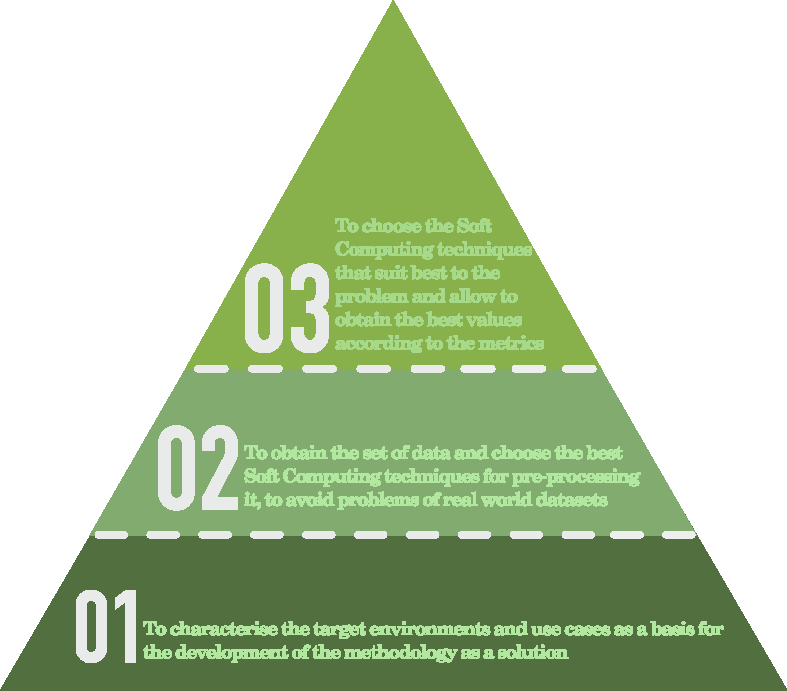
\includegraphics[scale =1.3] {gfx/intro/obj_pyramid.pdf}
\caption{Summary of the objectives of this thesis.}
\label{fig:pyramid}
\end{SCfigure}
